\documentclass[letter]{article}

\usepackage[english]{babel}
\usepackage[utf8]{inputenc}
\usepackage{amsmath}
\usepackage{graphicx}
\usepackage[colorinlistoftodos]{todonotes}
\usepackage{makecell}
\usepackage{multirow}
\usepackage{caption}
\usepackage{hyperref}
\hypersetup{colorlinks=true, pdfstartview=FitV, linkcolor=blue, citecolor=black, plainpages=false, pdfpagelabels=true, urlcolor=blue}
\usepackage[all]{hypcap}



% Adjust margins
\addtolength{\oddsidemargin}{-0.375in}
\addtolength{\evensidemargin}{-0.375in}
\addtolength{\textwidth}{1in}
\addtolength{\topmargin}{-.5in}
\addtolength{\textheight}{1.0in}

\title{CS 520: Assignment 1 - Path Planning and Search Algorithms}

\author{Shengjie Li}

\date{\today}

\begin{document}
\maketitle

\section{Introduction, group members and division of workload}
\label{sec:Introduction}

In this group project, apart from implementing DFS, BFS, A* with Euclidean Distance and A* with Manhattan Distance, we also did some modification to these algorithms for different performance out of our personal interests.  \\
\begin{tabular}{| p{2.5cm} | p{11.5cm} |}
	\hline
	\makecell[c]{Name \\ RUID} & Workload \\
	\hline
	\makecell[c]{Haoyang Zhang \\ 188008687} & {Implemented DFS, Iterative Deepening DFS, BFS, Bidirectional BFS, Beam Search, Simulated Annealing and the visualization of maze. Modified DFS to make it able to return optimal path. Added Last-in First-out feature to A*. Managed to combine Beam Search, Simulated Annealing and Genetic Algorithm. Ran tests for DFS and BFS in question 10. Finished half of the writing of report for part 2.} \\
	\hline
	\makecell[c]{Han Wu \\ 189008460} & {Wrote python scripts for testing the performance of algorithms. Got and Combine the data for question 1, 2, 4 and 5. Finished the writing of report for question 1, 2, 4 and 5.} \\
	\hline
	\makecell[c]{Shengjie Li \\ 188008047} & {Implemented A* with Euclidean Distance, A* with Manhattan Distance and Genetic Algorithm. Ran tests for A* with Euclidean Distance and Manhattan Distance inquestion 10. Finished the writing of whole report. } \\
	\hline
	\makecell[c]{Zhichao Xu \\ 188008912} & {Wrote python scripts for testing the performance of algorithms. Got and Combine the data for question 3, 6 and 7. Generated figures for questions in part 1. Finished the writing of report for question 3, 6 and 7. Suggested an improvement of A* using Chebyshev Distance.} \\
	\hline
\end{tabular}


\section{Part 1: Path Planning}
\label{sec:Part 1: Path Planning}

\begin{enumerate}
	\item {For each of the implemented algorithms, how large the maps can be ( in terms of dim ) for the algorithm to return an answer in a reasonable amount of time (less than a minute) for a range of possible p values? Select a size so that running the algorithms multiple times will not be a huge time commitment, but that the maps are large enough to be interesting.} \\
	The results are shown below as table \ref{table1}: \\
	\begin{center}
		\label{table1}
		\begin{tabular}[h]{| c | c | c | c | c | c | c | c |}
			\hline
			\multicolumn{2}{|c|}{} & \multicolumn{6}{c|}{Size} \\
			\cline{3-8}
			\multicolumn{2}{|c|}{} & 100 & 200 & 400 & 800 & 1600 & 3200 \\
			\hline
			\multirow{5}{*}{Time(s)} & DFS & 0.01942 & 0.07087 & 0.28435 & 0.93919 & 4.5064 & 10.83366 \\
			\cline{2-8}
			 & BFS\textsuperscript{2} & 0.07342 & 0.33946 & 1.73646 & 6.40967 & 25.69253 & 91.73234 \\
			 \cline{2-8}
			 & A* Euclidean & 0.07811 & 0.41706 & 1.62604 & 5.97804 & 25.27724 & 100.37974 \\
			 \cline{2-8}
			 & A* Manhattan & 0.06093 & 0.29222 & 0.88752 & 3.63068 & 11.147 & 63.8882 \\
			 \cline{2-8}
			 & BFS\textsuperscript{1} & \multicolumn{6}{l|}{254.36093 (size=30)} \\
			 \hline
		\end{tabular}
		\captionof{table}{}
	\end{center}
	DFS was the default setting. All conditions were false. BFS1 was the default setting. All conditions were False. However, it took too much time. When the size was 30, it took more than 250 seconds to return an answer. So, we changed the settings a little to make BFS acceptable. Here came BFS2. In BFS2, checkFringe was True. The others were also False. A* Euclidean means A* algorithm which used Euclidean Distance as the heuristic function. A* Manhattan means A Star algorithm which used Manhattan Distance as the heuristic function.
	
	In the table, we could see that when size becomes large, the average time of returning an answer (whether solvable or unsolvable) increases. BFS2 and A* Euclidean are often the most time-consuming algorithms. We need to run the algorithm for thousands of times (有待确认) in the following tests. In order to make it faster in the following test, we chose 200 as the default size of our maze.
	
	\item {Find a random map with $ p \approx 0.2 $ that has a path from corner to corner. Show the paths returned for each algorithm. (Showing maps as ASCII printouts with paths indicated is sufficient; however 20 bonus points are available for coding good visualizations.)}
	
	\item {For a fixed value of dim as determined in Question (1), for each $ p = 0.1, 0.2, 0.3, ... , 0.9 $, generate a number of maps and try to find a path from start to goal - estimate the probability that a random map has a complete path from start to goal, for each value of $ p $. Plot your data. Note that for $ p $ close to 0, the map is nearly empty and the path is clear; for $ p $ close to 1, the map is mostly filled and there is no clear path. There is some threshhold value $ p_0 $ so that for $ p < p_0 $ , there is usually a clear path, and $ p > p_0 $ there is no path. Estimate $ p_0 $ . Which path finding algorithm is most useful here, and why?}
	
\end{enumerate}


\subsection{Questions}
Here, explain the concept of a 2-DEG in GaAs/AlGaAs. What is a 2-DEG and why does it arise?

\subsection{Hall Effect}
Explain the classical Hall effect in your own words. What do I measure at $B=0$? And what happens if $B>0$? Which effect gives rise to the voltage drop in the vertical direction?

\subsection{Quantum Hall Effect}
Explain the IQHE in your own words. What does the density of states look like in a 2-DEG when $B=0$? What are Landau levels and how do they arise? What are edge states? What does the electron transport look like when you change the magnetic field? What do you expect to measure?

\section{Experiment 1-2 pages}
\subsection{Fabrication}
Explain a step-by-step recipe for fabrication here. How long did you etch and why? What is an Ohmic contact?
\subsection{Experimental set-up}
Explain the experimental set-up here. Use a schematic picture (make it yourself in photoshop, paint, ...) to show how the components are connected. Briefly explain how a lock-in amplifier works.

\section{Results and interpretation 2-3 pages}
Show a graph of the longitudinal resistivity ($\rho_{xx}$) and Hall resistivity ($\rho_{xy}$) versus magnetic field, extracted from the raw data shown in figure \ref{fig:data}. You will have the link to the data in your absalon messages, if not e-mail Guen (guen@nbi.dk). Explain how you calculated these values, and refer to the theory.

\begin{figure}
\centering
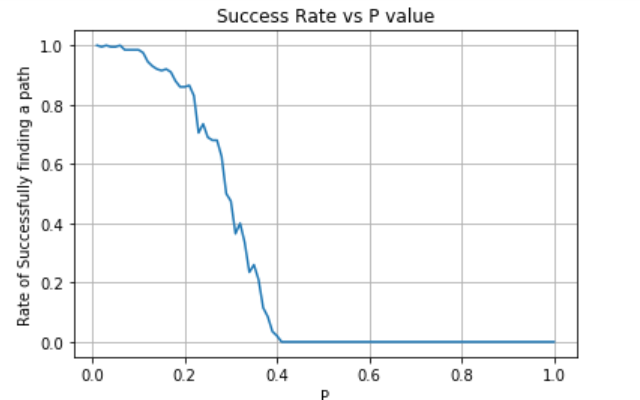
\includegraphics[width=1\textwidth]{../pics/question3-1.png}
\caption{\label{fig:data}Raw (unprocessed) data. Replace this figure with the one you've made, that shows the resistivity.}
\end{figure}

\subsection{Classical regime}
Calculate the sheet electron density $n_{s}$ and electron mobility $\mu$ from the data in the low-field regime, and refer to the theory in section \ref{sec:theory}. Explain how you retrieved the values from the data (did you use a linear fit?).
Round values off to 1 or 2 significant digits: 8.1643 ~= 8.2. Also, 5e-6 is easier to read than 0.000005.

!OBS: This part is optional (only if you have time left).
Calculate the uncertainty as follows: \newline $u(f(x, y, z)) = \sqrt{(\frac{\delta f}{\delta{x}} u(x))^{2} + (\frac{\delta f}{\delta{y}} u(y))^{2} + (\frac{\delta f}{\delta{z}} u(z))^{2}}$, where $f$ is the calculated value ($n_{s}$ or $\mu$), $x, y, z$ are the variables taken from the measurement and $u(x)$ is the uncertainty in x (and so on).

\subsection{Quantum regime}
Calculate $n_{s}$ for the high-field regime.
Show a graph of the longitudinal conductivity ($\rho_{xx}$) and Hall conductivity($\rho_{xy}$) \textbf{in units of the resistance quantum} ($\frac{h}{e^{2}}$), depicting the integer filling factors for each plateau.
Show a graph of the plateau number versus its corresponding value of $1/B$. From this you can determine the slope, which you use to calculate the electron density.
Again, calculate the uncertainty for your obtained values.

\section{Discussion 1/2-1 page}
Discuss your results. Compare the two values of $n_{s}$ that you've found in the previous section. Compare your results with literature and comment on the difference. If you didn't know the value of the resistance quantum, would you be able to deduce it from your measurements? If yes/no, why?

\newpage
\section{Some LaTeX tips}
\label{sec:latex}
\subsection{How to Include Figures}

First you have to upload the image file (JPEG, PNG or PDF) from your computer to writeLaTeX using the upload link the project menu. Then use the includegraphics command to include it in your document. Use the figure environment and the caption command to add a number and a caption to your figure. See the code for Figure \ref{fig:frog} in this section for an example.

\begin{figure}
\centering
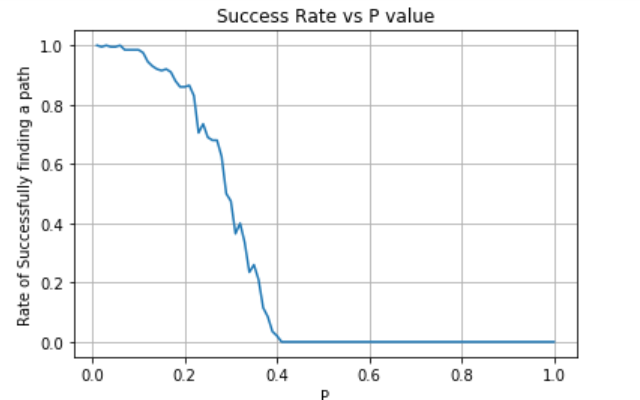
\includegraphics[width=0.3\textwidth]{../pics/question3-1.png}
\caption{\label{fig:frog}This frog was uploaded to writeLaTeX via the project menu.}
\end{figure}

\subsection{How to Make Tables}

Use the table and tabular commands for basic tables --- see Table~\ref{tab:widgets}, for example.

\begin{table}
\centering
\begin{tabular}{l|r}
Item & Quantity \\\hline
Widgets & 42 \\
Gadgets & 13
\end{tabular}
\caption{\label{tab:widgets}An example table.}
\end{table}

\subsection{How to Write Mathematics}

\LaTeX{} is great at typesetting mathematics. Let $X_1, X_2, \ldots, X_n$ be a sequence of independent and identically distributed random variables with $\text{E}[X_i] = \mu$ and $\text{Var}[X_i] = \sigma^2 < \infty$, and let

\begin{equation}
S_n = \frac{X_1 + X_2 + \cdots + X_n}{n}
      = \frac{1}{n}\sum_{i}^{n} X_i
\label{eq:sn}
\end{equation}

denote their mean. Then as $n$ approaches infinity, the random variables $\sqrt{n}(S_n - \mu)$ converge in distribution to a normal $\mathcal{N}(0, \sigma^2)$.

The equation \ref{eq:sn} is very nice.

\subsection{How to Make Sections and Subsections}

Use section and subsection commands to organize your document. \LaTeX{} handles all the formatting and numbering automatically. Use ref and label commands for cross-references.

\subsection{How to Make Lists}

You can make lists with automatic numbering \dots

\begin{enumerate}
\item Like this,
\item and like this.
\end{enumerate}
\dots or bullet points \dots
\begin{itemize}
\item Like this,
\item and like this.
\end{itemize}
\dots or with words and descriptions \dots
\begin{description}
\item[Word] Definition
\item[Concept] Explanation
\item[Idea] Text
\end{description}

We hope you find write\LaTeX\ useful, and please let us know if you have any feedback using the help menu above.

\begin{thebibliography}{9}
\bibitem{nano3}
  K. Grove-Rasmussen og Jesper Nygård,
  \emph{Kvantefænomener i Nanosystemer}.
  Niels Bohr Institute \& Nano-Science Center, Københavns Universitet

\end{thebibliography}
\end{document}